\chapter{Napoli DAQ}
\label{chap:napolidaq}

In this chapter, the Napoli DAQ will be explained. The codes for the plots are in \url{https://github.com/gm2-it/test-beam-slac-jun16/tree/master/NapoliDaq/analyzer}.

\section{Overview of the electronics}
A single Monitoring Board (MB) manages the entire signal processing for one of six Source Monitor (SM) elements. Light signals from the SM are opportunely divided among three channels: two PIN photodiodes and one PMT. 

The signal at the output of each photodetector is processed through a multistage electronics chain based on the following: (1) preamplifier; (2) pulse shaper; (3) baseline restorer; and (4) 14 bit analog to digital converter. The preamplifier circuit has been designed on a separate daughter board to allow for a custom, optimized interface for the specified sensor (PIN or PMT). 

For each channel the complete ADC readout and the control logic block are performed on a frontend FPGA where various slow control measurements (e.g. temperatures, bias voltage) are monitored. A 14 bit DAC on the same FPGA performs a self-calibration of the channel while a fourth, separate FPGA collects the signals from the three aforementioned FPGAs and communicates with the external interface, that is, provides the MB signals to the riders in order to be digitized.

\section{Data format}

Data is acquired in ASCII format, an example is shown in figure \ref{ASCII}.  Each line corresponds to an event and contains all the information readout by one of the three MB channels described previously. The data is recorded every time that one of the devices measures a signal that exceeds a fixed threshold. \\

\begin{figure}
\begin{center}
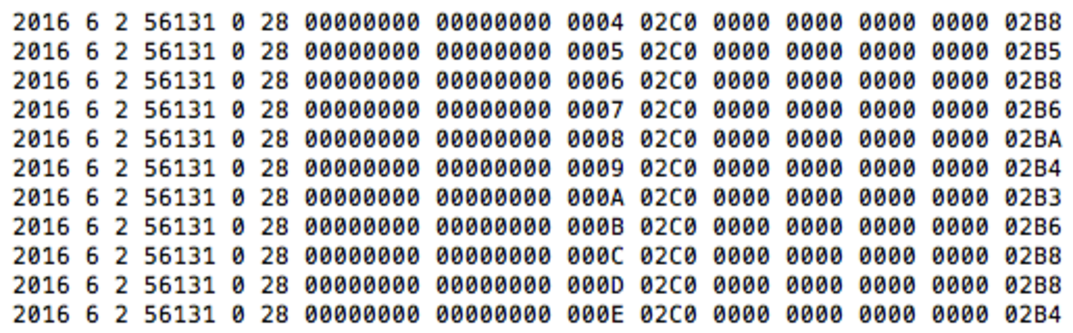
\includegraphics[width=\textwidth]{pics/NaDAQ.pdf}
\caption{Example of the ASCII files written by the Naples DAQ.}
\label{ASCII}
\end{center}
\end{figure}


\noindent For each event the following information (columns of figure \ref{ASCII}) is collected:
\begin{description}
  \item[1$^{st}$, 2$^{nd}$ and 3$^{rd}$ columns:] date (year, month and day) when the data are recorded (UTC time);
  \item[4$^{th}$ column:] time of the event ($i.e.$, the second of the day when the event happened);
 \item[5$^{th}$ column:] error code;
 \item[6$^{th}$ column:] number of bytes written;
 \item[7$^{th}$ column:] number of begin-of-fills;
 \item[8$^{th}$ column:] time in which the trigger occurred;
 \item[9$^{th}$ column:] number of triggers inside the fill;
 \item[10$^{th}$ column:] information about the MB and the signal (board address, channel, type of signal);
 \item[11$^{th}$, 12$^{th}$, 13$^{th}$ columns:] temperatures;
 \item[14$^{th}$ column:] information about the bias voltage of the device;
 \item[15$^{th}$ column:] charge of the signal.
\end{description} 

\subsection{From Raw Data to the ROOT tree}

Data, with the exception of the time, the error code and the space information (first six columns of fig. \ref{ASCII}) are recorded in hexadecimal. In order to make this data easy to analyze the raw data is converted into decimal numbers and stored in root files.
These root files are generated using the program that can be found here: \url{https://github.com/agioiosa/test-beam-slac-2016/tree/master/DAQ_Naples/SLAC2016Cruncher}.
The output of the program is a root file that contains a \verb+TTree+, named \verb+ntMonFrame+ with three branches: \verb+pmt+, \verb+pin1+ and \verb+pin2+. Each branch includes the following information:

\begin{description}
  \item \verb+ErrorCode+: is an error flag, if there are no errors it is set to be 0;
  \item \verb+frameloc+: is the numbers of bytes written. The expected value is 28, others numbers are an indication that an error is present;
  \item \verb+NBOF+: is the number of begin-of-fills occurred during the run (it is expected to be progressive);
\item \verb+NtrgBOF+: numbers of triggers during the fill;
 \item \verb+NTimeTrgBOF+: time of the trigger with respect to the time of the BOF;
\item	 \verb+PulseType+: set to be 1 in case of laser pulses and 2 in case of  americium pulses. 
\item \verb+BoardAdr+:  is the board address number (ranges from 0 to 11);
\item \verb+ChBoard+: mother board channel that acquired the data. There are 3 channels A, B, C  that correspond to 10, 11, 12, in decimal value. During the whole test beam, channel 10 was reading out the PMT and channels 11 and 12 the PIN1 and PIN2 outputs respectively;
\item \verb+boardTemp+: MB temperature readout by a probe that is close to the channel that is acquiring the event (each channel has its own temperature sensor);
\item \verb+cspTemp+: temperature of the preamplifier board related to the channel that is acquiring ($e.g.$, if ChBoard = 10, the cspTemp refers to the temperature of the PMT preamplifier board);
\item \verb+extTemp+: temperature of the probe connected to the channel. During the test beam at SLAC we used two of the three probes. For the position of the probes please refer to  UW elog post 78 [\url{https://muon.npl.washington.edu/elog/g2/SLAC+Test+Beam+2016/78}];
\item \verb+Vbias+: bias voltage of the device related to the acquiring channel;
\item \verb+ADCVal+: charge of the signal;
\item \verb+t_year+: temporal informations from rs232 board: year;
\item \verb+t_mon+: temporal informations from rs232 board: month;
\item \verb+t_day+: temporal informations from rs232 board: day;
\item \verb+t_secday+: temporal informations from rs232 board: seconds of day.
\end{description}

During this first stage, events with error code that differs from 0 are discarded. Events with other types of errors ($e.g.$, negative NBOF) might be still present and need to be removed during the further steps of the analysis. The decision of keeping also the ``bad'' events is supported by the fact that it is interesting to analyze the reason why the errors occurred and how they affect the data.

For the 2016 test beam at SLAC PulseType, cspTemp and one of the extTemp were not available.


\subsection{Example of an Analysis}

A preliminary off-line analysis of the data can be performed using the code posted in \url{https://github.com/agioiosa/test-beam-slac-2016/tree/master/DAQ_Naples/SLAC2016Ana}. The output of the code is a root file that contains the following plots:

\begin{description}
  \item[prof\_pmt\_ls\_adcval:]  charge of the laser pulse recorded by the PMT  as a function of the time measured in days;
  \item[prof\_pmt\_am\_adcval:] charge of the Am-pulse recorded by the PMT  as a function of the time measured in days;
  \item[h1\_pmt\_adcval:] histogram of the charge of the signals recorded by the PMT;
   \item[h2\_pmt\_nbof]  NBOF (recorded in the PMT channel) as a function of the time measured in days;
   \item[h1\_pmt\_ntimetrgbof] histogram of NTimeTrgBOF recorded in the PMT channel;
   \item[h2\_pmt\_ntimetrgbof] NTimeTrgBOF recorded in the PMT channel as a function of the time measured in days;
   \item[prof\_pmt\_vbias] PMT bias voltage as a function of the time measured in days;
   \item[prof\_pmt\_extemp] temperature measured by one of the external probes during the data acquisition;
   \item[prof\_pmt\_boardtemp:] temperature of the MB recorded in the PMT channel as a function of the time measured in days;
   \item[prof\_pin1\_adcval:]  charge of the laser pulse recorded by the PIN1  as a function of the time measured in days;
   \item[h1\_pin1\_adcval:] histogram of the charge of the signals recorded by the PIN1;
   \item[h2\_pin1\_nbof] NBOF (recorded in the PIN1 channel) as a function of the time measured in days;
   \item[h1\_pin1\_ntimetrgbof] histogram of NTimeTrgBOF recorded in the PIN1 channel;  
   \item[h2\_pin1\_ntimetrgbof]  NTimeTrgBOF recorded in the PIN1 channel as a function of the time measured in days;
   \item[prof\_pin1\_vbias:] PIN1 bias voltage as a function of the time measured in days;
   \item[prof\_pin1\_extemp:]  temperature measured by one of the external probes during the data acquisition;
   \item[prof\_pin1\_boardtemp:]  temperature of the MB recorded in the PIN1 channel as a function of the time measured in days;   
   \item[prof\_pin2\_adcval:]  charge of the laser pulse recorded by the PIN2  as a function of the time measured in days;
   \item[h1\_pin2\_adcval:] histogram of the charge of the signals recorded by the PIN2;
   \item[h2\_pin2\_nbof:] NBOF (recorded in the PIN2 channel) as a function of the time measured in days;
   \item[h1\_pin2\_ntimetrgbof:] histogram of NTimeTrgBOF recorded in the PIN2 channel;
   \item[h2\_pin2\_ntimetrgbof:]  NTimeTrgBOF recorded in the PIN2 channel as a function of the time measured in days;
   \item[prof\_pin2\_extemp:] PIN2 bias voltage as a function of the time measured in days;
   \item[prof\_pin2\_boardtemp:] temperature of the MB recorded in the PIN2 channel as a function of the time measured in days;
   \item[prof\_pin1Dpin2\_adcval:] ratio between the signal recorded by the PINs as a function of the time measured in days;
   \item[h1\_pin1Dpin2\_adcval:]  ratio between the signal recorded by the PINs;	
   \item[h1\_ratio\_pin1\_pin2\_adcval:]  histogram of the ratio between the signal recorded by the PINs;
   \item[h2\_pin1Vpin2\_adcval:]  correlation between PIN1 and PIN2 signals;  
     %\item[prof\_pmt\_ls\_am\_ratio:]  ratio between laser and americium pulses recorded by the PMT  as a function of the time measured in days;	
       	\item[h1\_lsDam\_adcval:]  histogram of the ratio between laser and americium pulses recorded by the PMT.	
\end{description}


Temperatures are recorded in arbitrary units ($temp$) and then transformed into degrees Celsius by using the following relation: $temp \cdot 200/2047-50$.


